% Options for packages loaded elsewhere
\PassOptionsToPackage{unicode}{hyperref}
\PassOptionsToPackage{hyphens}{url}
%
\documentclass[
]{article}
\usepackage{lmodern}
\usepackage{amsmath}
\usepackage{ifxetex,ifluatex}
\ifnum 0\ifxetex 1\fi\ifluatex 1\fi=0 % if pdftex
  \usepackage[T1]{fontenc}
  \usepackage[utf8]{inputenc}
  \usepackage{textcomp} % provide euro and other symbols
  \usepackage{amssymb}
\else % if luatex or xetex
  \usepackage{unicode-math}
  \defaultfontfeatures{Scale=MatchLowercase}
  \defaultfontfeatures[\rmfamily]{Ligatures=TeX,Scale=1}
\fi
% Use upquote if available, for straight quotes in verbatim environments
\IfFileExists{upquote.sty}{\usepackage{upquote}}{}
\IfFileExists{microtype.sty}{% use microtype if available
  \usepackage[]{microtype}
  \UseMicrotypeSet[protrusion]{basicmath} % disable protrusion for tt fonts
}{}
\makeatletter
\@ifundefined{KOMAClassName}{% if non-KOMA class
  \IfFileExists{parskip.sty}{%
    \usepackage{parskip}
  }{% else
    \setlength{\parindent}{0pt}
    \setlength{\parskip}{6pt plus 2pt minus 1pt}}
}{% if KOMA class
  \KOMAoptions{parskip=half}}
\makeatother
\usepackage{xcolor}
\IfFileExists{xurl.sty}{\usepackage{xurl}}{} % add URL line breaks if available
\IfFileExists{bookmark.sty}{\usepackage{bookmark}}{\usepackage{hyperref}}
\hypersetup{
  pdftitle={Maintainance of Certification and Medicare Outcomes},
  pdfauthor={Xilin Chen},
  hidelinks,
  pdfcreator={LaTeX via pandoc}}
\urlstyle{same} % disable monospaced font for URLs
\usepackage[margin=1in]{geometry}
\usepackage{graphicx}
\makeatletter
\def\maxwidth{\ifdim\Gin@nat@width>\linewidth\linewidth\else\Gin@nat@width\fi}
\def\maxheight{\ifdim\Gin@nat@height>\textheight\textheight\else\Gin@nat@height\fi}
\makeatother
% Scale images if necessary, so that they will not overflow the page
% margins by default, and it is still possible to overwrite the defaults
% using explicit options in \includegraphics[width, height, ...]{}
\setkeys{Gin}{width=\maxwidth,height=\maxheight,keepaspectratio}
% Set default figure placement to htbp
\makeatletter
\def\fps@figure{htbp}
\makeatother
\setlength{\emergencystretch}{3em} % prevent overfull lines
\providecommand{\tightlist}{%
  \setlength{\itemsep}{0pt}\setlength{\parskip}{0pt}}
\setcounter{secnumdepth}{-\maxdimen} % remove section numbering
\usepackage{booktabs}
\usepackage{longtable}
\usepackage{array}
\usepackage{multirow}
\usepackage{wrapfig}
\usepackage{float}
\usepackage{colortbl}
\usepackage{pdflscape}
\usepackage{tabu}
\usepackage{threeparttable}
\usepackage{threeparttablex}
\usepackage[normalem]{ulem}
\usepackage{makecell}
\usepackage{xcolor}
\ifluatex
  \usepackage{selnolig}  % disable illegal ligatures
\fi

\title{Maintainance of Certification and Medicare Outcomes}
\usepackage{etoolbox}
\makeatletter
\providecommand{\subtitle}[1]{% add subtitle to \maketitle
  \apptocmd{\@title}{\par {\large #1 \par}}{}{}
}
\makeatother
\subtitle{Cohort Definition}
\author{Xilin Chen}
\date{2021-06-01}

\begin{document}
\maketitle

{
\setcounter{tocdepth}{3}
\tableofcontents
}
This document describes how the ABS maintenance of certification and
medicare outcomes cohort was defined. The data will be used for further
statistical analyses.

\hypertarget{data-sources}{%
\subsection{1. Data Sources}\label{data-sources}}

\begin{itemize}
\tightlist
\item
  ABS certification data (received at September 2019 from ABS)
\item
  Fellowship Council data (\textbf{Need to incorporate Angie's updates
  from Bariatric project})
\item
  Medicare claim data

  \begin{itemize}
  \tightlist
  \item
    Year: 2007-2018
  \item
    Procedures: commonly performed general surgery procedures (162
    procedures in total)
  \end{itemize}
\end{itemize}

ABS and Medicare claim data are linked using physician NPIs. ABS and
Fellowship council data are used to exclude fellowship trained surgeons.

\pagebreak

\hypertarget{cohort-definition-diagram-overview}{%
\subsection{2. Cohort definition diagram
overview}\label{cohort-definition-diagram-overview}}

Below is the consort diagram for the data selection process. Detailed
cohort selection descriptions are included in \emph{3. Data Process} and
\emph{4. Data linkage}.

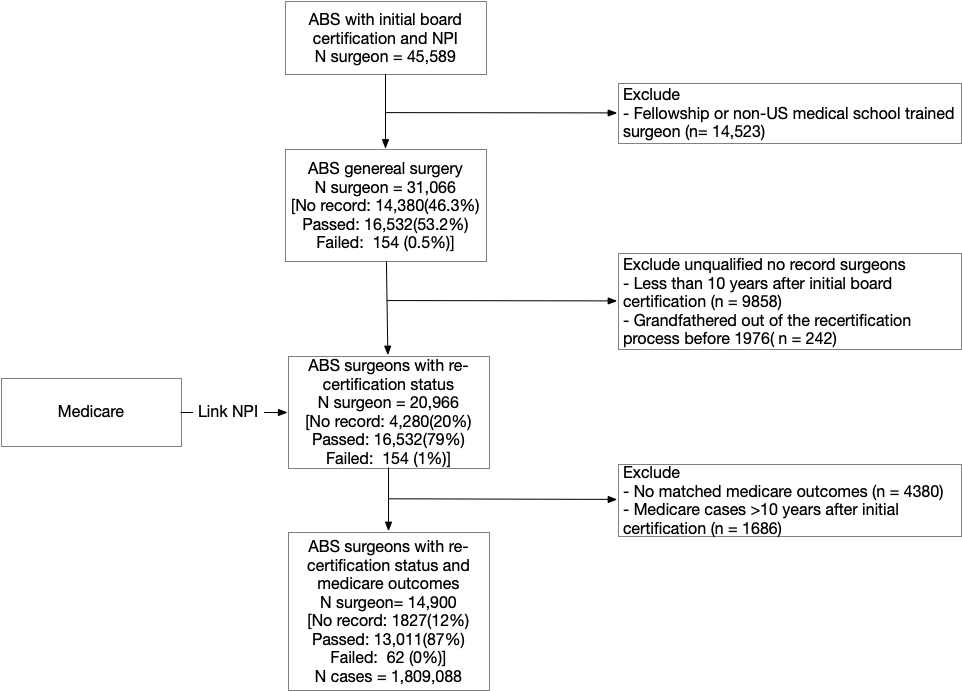
\includegraphics{/Users/xilinchen/Documents/Repo/ABS_MoC_vs_pt_Outcome/other_docs/Diagram/cohort_definition/cohort_definition.png}

\hypertarget{data-process}{%
\subsection{3. Data Process}\label{data-process}}

\hypertarget{abs}{%
\subsubsection{ABS}\label{abs}}

\hypertarget{inclusion-and-exclusion}{%
\subsubsection{3.1. Inclusion and
Exclusion}\label{inclusion-and-exclusion}}

Inclusion:

\begin{itemize}
\tightlist
\item
  Surgeons with NPI
\item
  Passed initial certification exam after 1976
\item
  ABS introduced time-limited MOC certification in 1976. So we we only
  include surgeons who pass their initial certification after 1976. This
  is also described in Andrew Jones MOC paper, \emph{Certification data
  were collected from the ABS database for all surgeons initially
  certified in general surgery by the ABS between 1976 and 2005}.
\item
  Not qualified (10 years after initial certification) for exam after
  2017 (exam change in 2017)

  \begin{itemize}
  \tightlist
  \item
    to address the exam changes in 2017, we excluded all surgeons who
    were qualified for recertification after(including) 2017. In our
    dataset, we don't have the recertifcation exam years for surgeons.
    So it's not possible to know if the surgeon took the exam before or
    after 2017. By excluding surgeons who were qualified to take the
    exam after 2017, we exclude the group who might have taken the exam
    after 2017. However, this also excluded some surgeons who took
    recertification exam earlier than 10 years after the initial
    certification.
  \end{itemize}
\end{itemize}

Exclusion:

\begin{itemize}
\tightlist
\item
  Fellowship or non-US trained surgeons (n = 16472).

  \begin{itemize}
  \tightlist
  \item
    Fellowship and Med school information is from ABS and Fellowship
    Council data.
  \end{itemize}
\end{itemize}

Below is the re-certification status for all qualified ABS surgeons.
Very few surgeons have recorded failed re-certification status. A large
portion of surgeons didn't have re-certification records at all,
i.e.~NA.

\begin{table}[H]
\centering
\begin{tabular}{l|r|l}
\hline
Recert\_status & n suregon & percentage\\
\hline
failed & 136 & 1\%\\
\hline
NA\_failed & 3982 & 20\%\\
\hline
passed & 15671 & 79\%\\
\hline
\end{tabular}
\end{table}

\hypertarget{data-linkage}{%
\subsection{4. Data linkage}\label{data-linkage}}

\hypertarget{link-medicare-data-with-abs-data-by-npi}{%
\subsubsection{4.1 Link Medicare data with ABS data by
NPI}\label{link-medicare-data-with-abs-data-by-npi}}

\hypertarget{only-keep-cases-that-performed-between-10-20-years-after-initial-certification}{%
\subsubsection{4.2 Only keep cases that performed between 10-20 years
after initial
certification*}\label{only-keep-cases-that-performed-between-10-20-years-after-initial-certification}}

The ABS gives 10 years for surgeons for the recertification. We keep
cases that 10 years after the initial certification to better capture
the impact of the recertification process. However, we excluded cases
happened 20 years after the initial certification to exlude the
re-recertification effect,.e. only the first recertification cases were
included in the cohort.

Link ABS with Medicare by NPI. Below is the number of surgeons by each
recertification category after linked with Medicare outcomes.

\begin{table}[H]
\centering
\begin{tabular}{l|r|l}
\hline
Recert\_status & n suregon & percentage\\
\hline
failed & 44 & 0\%\\
\hline
NA\_failed & 1173 & 11\%\\
\hline
passed & 9597 & 89\%\\
\hline
\end{tabular}
\end{table}

4475 ABS surgeons don't have Medicare cases matched; 4500 surgeons don't
have cases between 10 to 20 years after the initial certification.

\hypertarget{qa}{%
\subsection{5. Q\&A}\label{qa}}

5.1 Did we exclude surgeons who didn't have enough time to pass
Recertification exam? For example, if a surgeon only had 8 years after
the initial certification, would the surgeon be excluded for the
analysis?

In our study, we only included surgeons who were initially board
certified before 2007. We have ABS data available up to 2019. So every
surgeon in our study had at least 12 years of record after initial
certification. ABS requires recertification every 10 years.

5.2 What if a surgeon passed the exam at year 12 after the initial
certification? Would the surgeon be excluded because s/he didn't get
certified within 10 years?

The surgeon is included. No criteria was about when the surgeon was
re-certified. The recertified data we have is binary, without any year
information of when the surgeons took the exam. So we can't know if the
recertification was on-time or late.

5.3 Examples of how the recertification status were defined.

\begin{table}[H]
\centering
\begin{tabular}{l|r|r|l}
\hline
npi & Gcertyear & ReCeverPassed & Recert\_status\\
\hline
surgeon 1 & 1977 & 0 & failed\\
\hline
surgeon 2 & 1992 & 0 & failed\\
\hline
surgeon 3 & 2006 & 0 & failed\\
\hline
surgeon 4 & 1984 & 0 & failed\\
\hline
surgeon 5 & 2006 & 0 & failed\\
\hline
surgeon 6 & 2005 & NA & NA\_failed\\
\hline
surgeon 7 & 1979 & NA & NA\_failed\\
\hline
surgeon 8 & 1995 & NA & NA\_failed\\
\hline
surgeon 9 & 1987 & NA & NA\_failed\\
\hline
surgeon 10 & 2006 & NA & NA\_failed\\
\hline
surgeon 11 & 1983 & 1 & passed\\
\hline
surgeon 12 & 1989 & 1 & passed\\
\hline
surgeon 13 & 2003 & 1 & passed\\
\hline
surgeon 14 & 1995 & 1 & passed\\
\hline
surgeon 15 & 2001 & 1 & passed\\
\hline
\end{tabular}
\end{table}

\begin{itemize}
\tightlist
\item
  Gcertyear: year of initial board certification; ReCeverPassed:
  Original ABS variable 0 (failed), 1 (passed)
\end{itemize}

\end{document}
